% !TEX encoding = UTF-8 Unicode

\documentclass[a4paper]{article}
\usepackage[margin=2.5cm]{geometry}

\usepackage{color}
\usepackage{url}
\usepackage[T2A]{fontenc} % enable Cyrillic fonts
\usepackage[utf8x]{inputenc} % make weird characters work
\usepackage{graphicx}
\usepackage{caption}
\usepackage{subcaption}
\usepackage{float}
\usepackage[section]{placeins}
\usepackage[english,serbian]{babel}
\usepackage{color}
%\usepackage[english,serbianc]{babel} %ukljuciti babel sa ovim opcijama, umesto gornjim, ukoliko se koristi cirilica

\usepackage[unicode]{hyperref}
\hypersetup{colorlinks,citecolor=green,filecolor=green,linkcolor=blue,urlcolor=blue}

%\newtheorem{primer}{Пример}[section] %ćirilični primer
\newtheorem{definicija}{Definicija}[section]

\begin{document}

\title{ATP 2000-2017\\ \small{Seminarski rad u okviru kursa\\Istraživanje podataka\\ Matematički fakultet\\} \vspace{1cm}}
\author{Marija Mijailović\\mi14199@alas.matf.bg.ac.rs\\ \\Miroslav Mišljenović\\mr12260@alas.matf.bg.ac.rs}
\date{jun 2018.}
\maketitle

\abstract{
U ovom radu analizirali smo skup podataka ˝ATP - rezultati turnira od 2000-2017˝. Obradili smo pravila pridruživanja, klasterovanje, klasifikaciju i predstavili sve navedene metode odgovarajućom vizualizacijom. Skup podataka je preuzet sa \url{https://www.kaggle.com/gmadevs/atp-matches-dataset}.
}

\tableofcontents

\newpage

\newgeometry{top=4.0cm}
\section{Uvod}
\label{sec:uvod}

Skup podataka ATP mečeva podeljen je u 17 zasebnih .csv fajlova i svaki od njih prikazuje individualne statistike za svaki turnir u toku te godine.

\section{Analiza podataka}

U ovom poglavlju sledi kratak pregled najistaknutijih atributa ovog skupa podataka.
Svaki red u skupu, označava jedan meč i sve informacije o tom meču.

U tabeli \ref{table:turnir} prikazani su podaci o turniru.


\begin{table}[H]
	\begin{center}
		\begin{tabular}{ | c | c | } 
			\hline
			Ime kolone & Objašnjenje \\ 
			\hline
			tourney\_id & id turnira \\
			tourney\_name & ime turnira \\
			surface & podloga(Grass, Clay, Hard) \\
			tourney\_level & nivo turnira(Grand Slam, Finals, Masters, Tour Series, Challenger) \\ 
			round & runda(Round of 16, Quarterfinal...) \\
			minutes & trajanje meča u minutima \\
			\hline
		\end{tabular}
	\end{center}
	\caption{Podaci o turnirima}
	\label{table:turnir}
\end{table}

U tabeli \ref{table:pobednici} prikazani su podaci o pobedniku meča.
\begin{table}[H]
	\begin{center}
		\begin{tabular}{ | c | c | } 
			\hline
			Ime kolone & Objašnjenje \\ 
			\hline
			winner\_seed & nosilac na turniru \\
			winner\_entry & ulaznica(WildCard, Qualified, LuckyLoser, ProtectedRanking) \\
			winner\_name & ime pobednika \\
			winner\_ht & visina pobednika \\
			winner\_ioc & zemlja porekla pobednika \\
			winner\_age & godine pobednika \\
			winner\_rank & ATP rang pobednika \\
			winner\_rank\_points & ATP poeni pobednika \\
			w\_ace & broj asova pobednika \\
			w\_df & broj duplih grešaka pobednika \\ 
			w\_svpt & broj poena dobijenih na servis pobednika \\
			w\_1stIn & broj ubačenih prvih servisa pobednika \\
			w\_1stWon & broj poena dobijenih nakon ubačenog prvog servisa pobednika \\
			w\_2ndWon & broj poena dobijenih nakon ubačenog drugog servisa pobednika \\
			w\_SvGms & broj gemova u kojima je servirao pobednik \\
			w\_bpSaved & broj spašenih brejk šansi pobednika \\
			w\_bpFaced & broj brejk šansi na servis pobednika \\ 
			\hline
		\end{tabular}
	\end{center}
	\caption{Podaci o pobednicima}
	\label{table:pobednici}
\end{table}

\restoregeometry
U tabeli \ref{table:gubitnici} prikazani su podaci o gubitniku meča.
\begin{table}[H]
	\begin{center}
		\begin{tabular}{ | c | c | } 
			\hline
			Ime kolone & Objašnjenje \\ 
			\hline
			loser\_seed & nosilac na turniru \\
			loser\_entry & ulaznica(WildCard, Qualified, LuckyLoser, ProtectedRanking) \\
			loser\_name & ime gubitnika \\
			loser\_ht & visina gubitnika \\
			loser\_ioc & zemlja porekla gubitnika \\
			loser\_age & godine gubitnika \\
			loser\_rank & ATP rang gubitnika \\
			loser\_rank\_points & ATP poeni gubitnika \\ 
			l\_ace & broj asova gubitnika \\
			l\_df & broj duplih grešaka gubitnika \\
			l\_svpt & broj poena dobijenih na servis gubitnika \\
			l\_1stIn & broj ubačenih prvih servisa gubitnika \\
			l\_1stWon & broj poena dobijenih nakon ubačenog prvog servisa gubitnika \\
			l\_2ndWon & broj poena dobijenih nakon ubačenog drugog servisa gubitnika \\
			l\_SvGms & broj gemova u kojima je servirao gubitnik \\
			l\_bpSaved & broj spašenih brejk šansi gubitnika \\
			l\_bpFaced & broj brejk šansi na servis gubitnika \\
			\hline
		\end{tabular}
	\end{center}
	\caption{Podaci o gubitnicima}
	\label{table:gubitnici}
\end{table}

S obzirom na veliki broj raspoloživih godina, prvo smo se detaljno upoznali sa podacima, šta nam koja godina pruža i koji su najzanimljiviji atributi za svaku godinu. U zavisnosti od toga smo, po potrebama metoda, koristili različite godine, ali svuda smo se ograničili na četiri maksimalno.

\section{Pravila pridruživanja}

Pravila pridruživanja smo obradili u programskom alatu KNIME (slika \ref{fig:knime}).
Odlučili smo se za 2009. godinu, jer su rezultati reprezentativniji u odnosu na ostale godine.

\begin{figure}[H]
	\begin{center}
		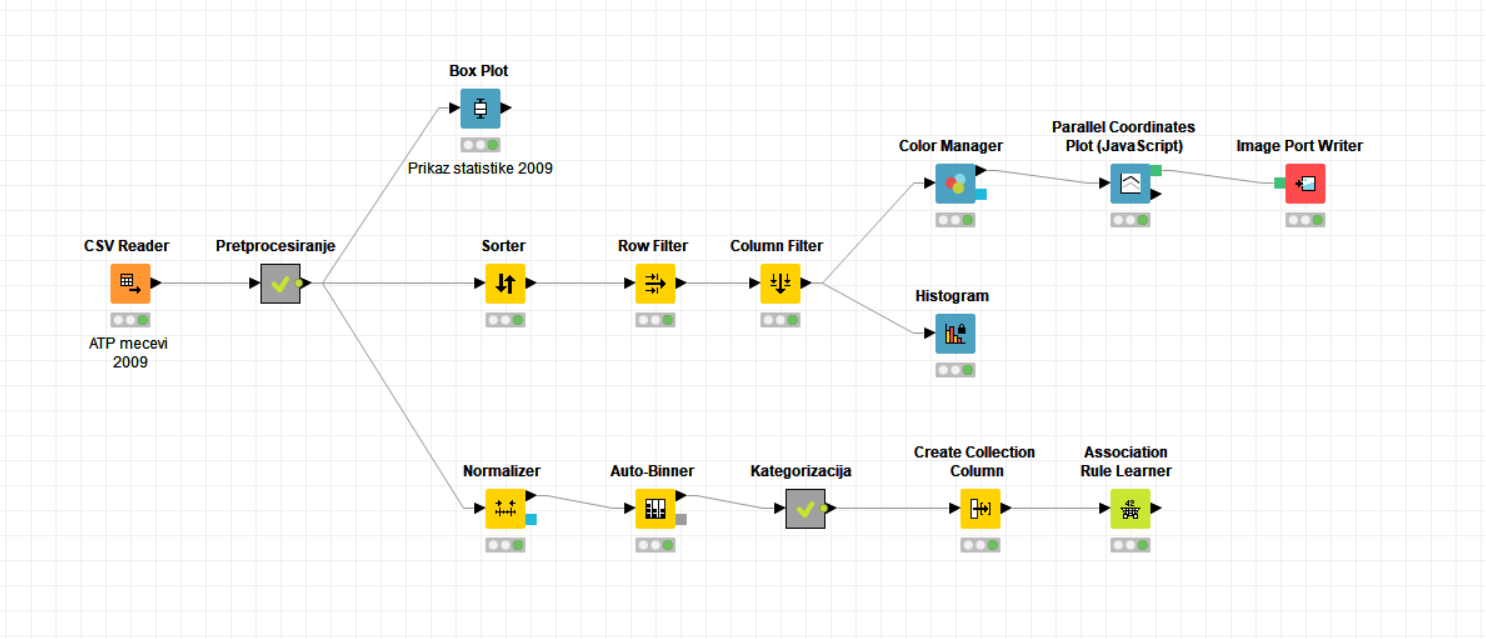
\includegraphics[width=1\textwidth]{PravilaPridruzivanja/knime.png}
	\end{center}
	\caption{KNIME implementacija}
	\label{fig:knime}
\end{figure}

Na slikama \ref{fig:histogram} i \ref{fig:parallel} grafički su prikazani rezultati za sedam
tenisera koji su imali prosečno najviše asova po meču na kome su pobedili. Izabrali smo četiri parametra za svakog igrača:
broj asova pobednika, broj dobijenih poena na servis pobednika, broj ubačenih prvih servisa pobednika i
broj osvojenih poena nakon ubačenog prvog servisa pobednika. Na histogramu i grafiku paralelnih koordinata 
mogu se videti i uporediti rezultati.

\begin{figure}[H]
	\begin{center}
		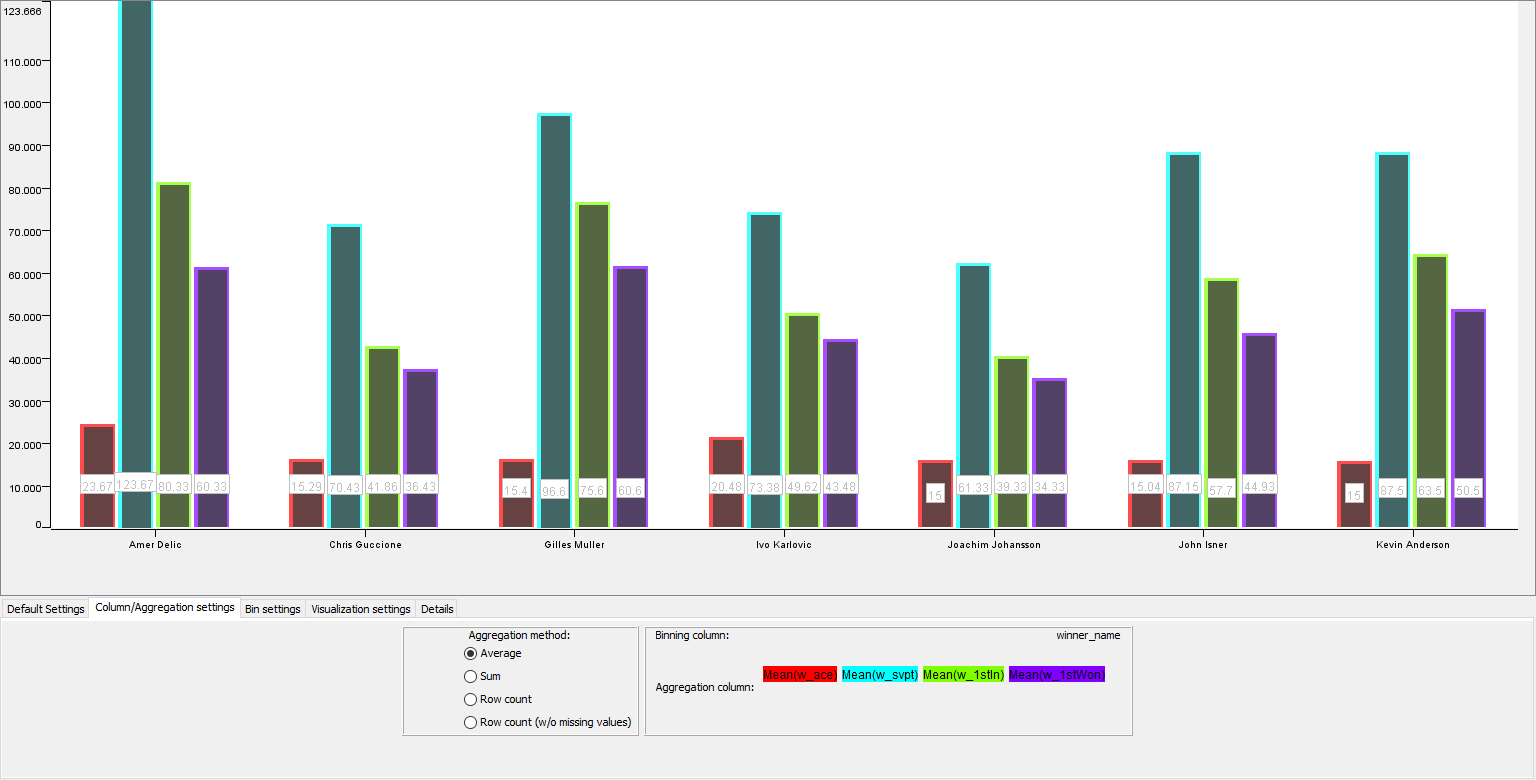
\includegraphics[width=1\textwidth]{PravilaPridruzivanja/histogram2009}
	\end{center}
	\caption{Histogram}
	\label{fig:histogram}
\end{figure}

\begin{figure}[H]
	\begin{center}
		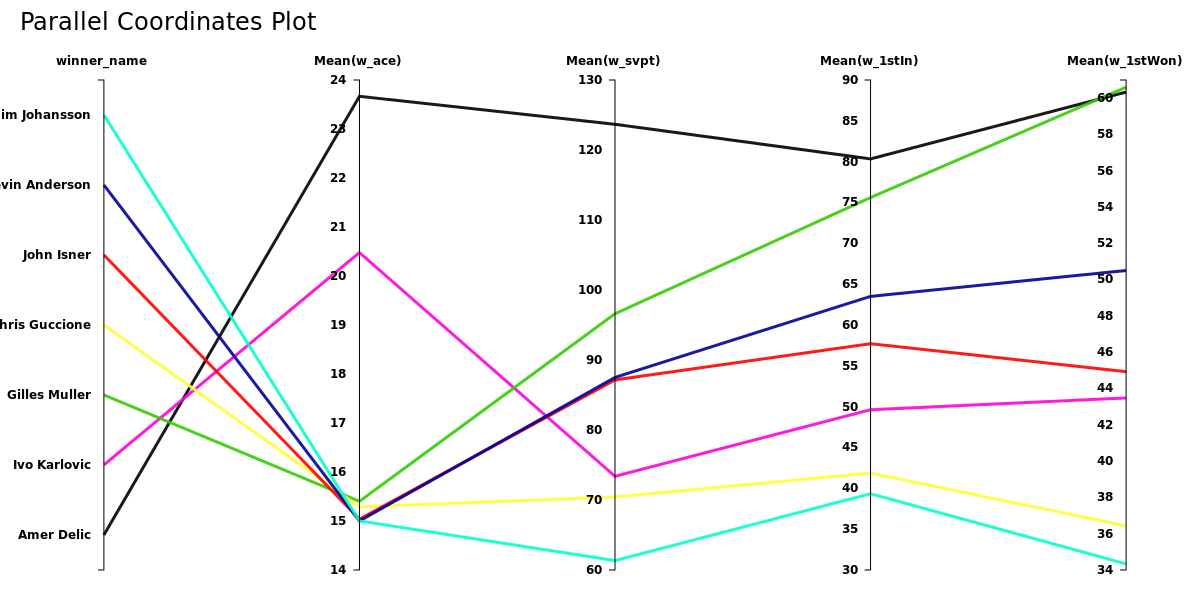
\includegraphics[width=1\textwidth]{PravilaPridruzivanja/parallel2009}
	\end{center}
	\caption{Paralelne koordinate}
	\label{fig:parallel}
\end{figure}

Iznenađenje je pojavljivanje Amera Delića u prvih sedam, jer je to
autorima nepoznat igrač. Uvidom u podatke, utvrđeno je da je on te godine odigrao samo osam mečeva,
a pobedio je samo tri puta, u mečevima u kojima je imao mnogo asova (što je kriterijum po kome je birano najboljih sedam). \\

U tri kategorije smo podelili sledeća četiri atributa: broj asova pobednika, broj duplih servis grešaka pobednika,
broj osvojenih poena nakon ubačenog prvog servisa pobednika, broj spašenih brejk lopti pobednika.
Na slici \ref{fig:rule_learner} se mogu videti pravila pridruživanja dobijena na osnovu te kategorizacije,
sortirani po Lift meri. Za pouzdanost smo uzeli vrednost 0.4, a za minimalnu podršku vrednost 0.15.
Analizirali smo podatke za sve godine i rezultati su prilično uniformni. Za 2009. godinu je dobijena druga najveća
Lift mera (1.36) i odnosi se na pravilo [ACE 2, WON 2, DF 1] -> [BPS 1].
U 2004. godini smo dobili najveću vrednost Lift mere (1.441) za pravilo [BPS 1, ACE 1, DF 1] -> [WON 1].

\newgeometry{top=6.0cm}
\begin{figure}[H]
	\begin{center}
		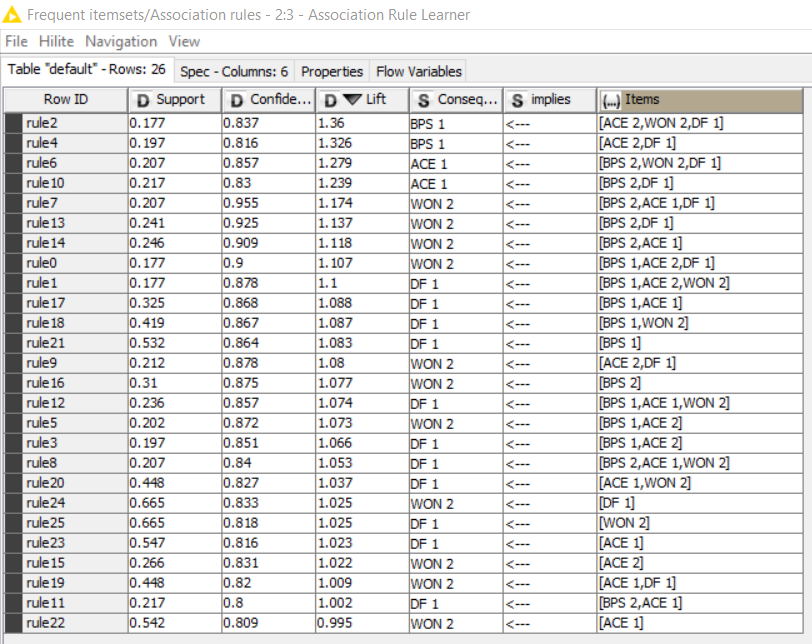
\includegraphics[width=1\textwidth]{PravilaPridruzivanja/rule_learner_2009}
	\end{center}
	\caption{Pravila pridruživanja za 2009. godinu}
	\label{fig:rule_learner}
\end{figure}

\section{Klasterovanje}

Što se tiče klasterovanja, s obzirom da podaci po godinama dosta osciliraju, odlučili smo da klasterovanje izvršimo za više godina. Izabrali smo 2003., 2011. i 2017. godinu. Pre svega, zanimala nas je zavisnost broja godina pobednika i broj asova pobednika. Prvo smo obradili nedostajuće vrednosti. Klasterovanje smo obradili u alatima SPSS i KNIME (slike \ref{fig:SPSS_CvoroviKlasterovanje} i \ref{fig:KNIME_CvoroviKlasterovanje}). 

\restoregeometry
\subsection{SPSS}

\begin{figure}[H]
	\begin{center}
		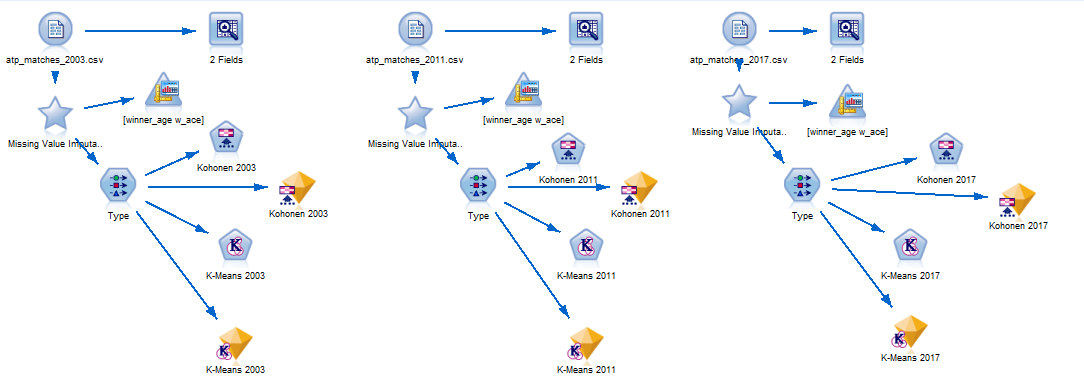
\includegraphics[scale=0.4]{Klasterovanje/SPSS_Cvorovi.png}
	\end{center}
	\caption{SPSS klasterovanje}
	\label{fig:SPSS_CvoroviKlasterovanje}
\end{figure}

\newgeometry{top=5.0cm}
U alatu SPSS smo pomoću siluete pratili kako nam se kvalitet klasterovanja razlikuje u zavisnosti od broja klastera. 
\textit{Kohonen} algoritam nam je za broj klastera između 3 i 5 davao ˝osrednji˝ kvalitet klasterovanja, pa ga nismo detaljno razmatrali. S druge strane, \textit{K-Means} algoritam nam je davao dosta raznolike ocene klastera po godinama. 2003. godina nam je za 4 i 5 klastera pokazala kvalitet klasterovanja  ˝dobar˝, uz važnost atributa \textit{w\_age = 1} i \textit{w\_ace = 1}. U 2011. godini nam je za 5 klastera silueta pokazivala kvalitet ˝osrednji˝, promenivši broj klastera na 4 silueta je prešla u ˝dobar˝. Takođe, i sa 4 klastera i sa 5 klastera važnost atributa \textit{w\_age = 1} i \textit{w\_ace = 1}. Rezultati za 2017. godinu za 4 klastera pokazuju kvalitet ˝osrednji˝; promenivši broj klastera na 5, silueta je na granici ˝osrednji˝-˝dobar˝, međutim, važnost atributa sa 4 klastera je \textit{w\_age = 1}, \textit{w\_ace = 0.77}, dok je sa 5 klastera \textit{w\_ace} opao na 0.46. Ipak smo odlučili da 2017. godinu odbradimo sa 5 klastera. Konačno, odlučili smo se za broj i kvalitet klastera koji su prikazani na slikama \ref{fig:SPSS_Silueta2003}, \ref{fig:SPSS_Silueta2011} i \ref{fig:SPSS_Silueta2017}.

\vspace{2cm}
\begin{figure}[H]
	\begin{center}
		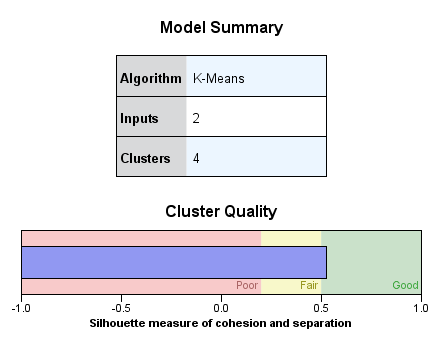
\includegraphics[width=0.7\textwidth]{Klasterovanje/Model_KMeans2003_Silhouette.png}
	\end{center}
	\caption{Kvalitet klasterovanja - 2003. godina}
	\label{fig:SPSS_Silueta2003}
\end{figure}

\restoregeometry
\begin{figure}[H]
	\begin{center}
		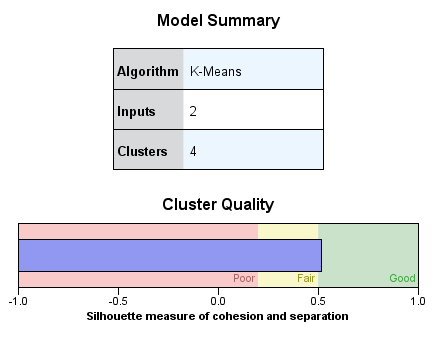
\includegraphics[width=0.7\textwidth]{Klasterovanje/Model_KMeans2011_Silhouette.png}
	\end{center}
	\caption{Kvalitet klasterovanja - 2011. godina}
	\label{fig:SPSS_Silueta2011}
\end{figure}

\begin{figure}[H]
	\begin{center}
		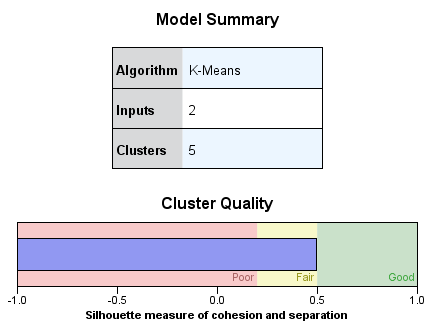
\includegraphics[width=0.7\textwidth]{Klasterovanje/Model_KMeans2017_Silhouette.png}
	\end{center}
	\caption{Kvalitet klasterovanja - 2017. godina}
	\label{fig:SPSS_Silueta2017}
\end{figure}

Kao što se vidi na slici \ref{ModeliKlastera}, u sve tri godine su dobijeni interesantni podaci. Na primer, u 2003. godini najstariji igrači imaju slabiji prosek asova, dok u 2011. i 2017. godini imamo dva klastera sa prosekom godina oko 30; u jednom klasteru nam je broj asova mali, dok je u drugom najveći. Ovo nam je govorilo da možda imamo neki element van granica, koji je uticao na kreiranje dodatnog klastera. Odlučili smo da proverimo šta ćemo dobiti u KNIME-u.

\begin{figure}[H]
	\begin{subfigure}[h]{\textwidth}
		\begin{center}
			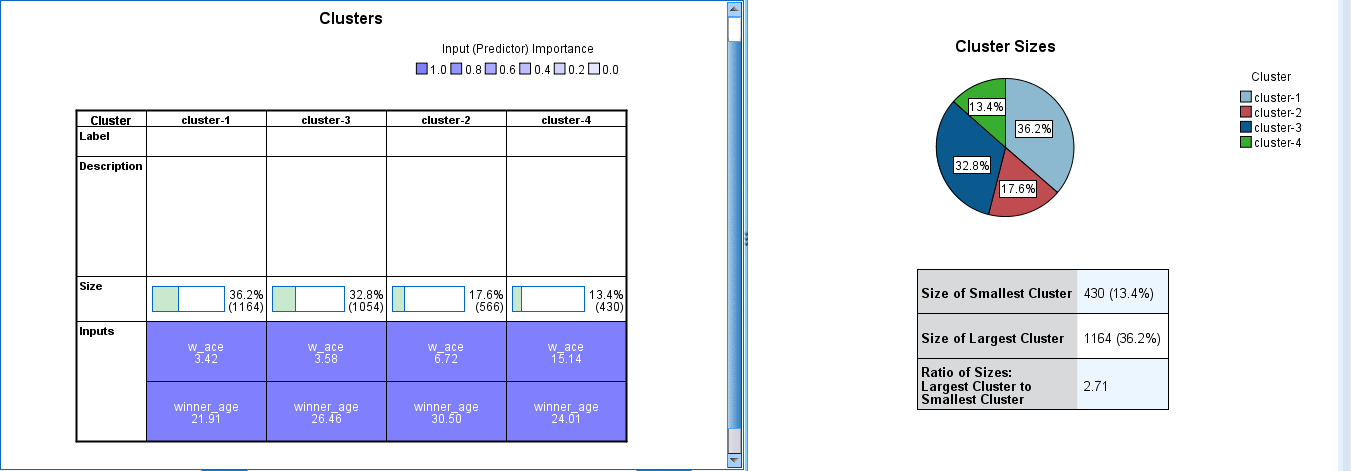
\includegraphics[scale=0.60]{Klasterovanje/Model_KMeans2003.png}
		\end{center}
		\caption{2003. godina}
		\label{fig:SPSS_Model2003}
	\end{subfigure}
	
	\vspace{0.5cm}
	\begin{subfigure}[h]{\textwidth}
		\begin{center}
			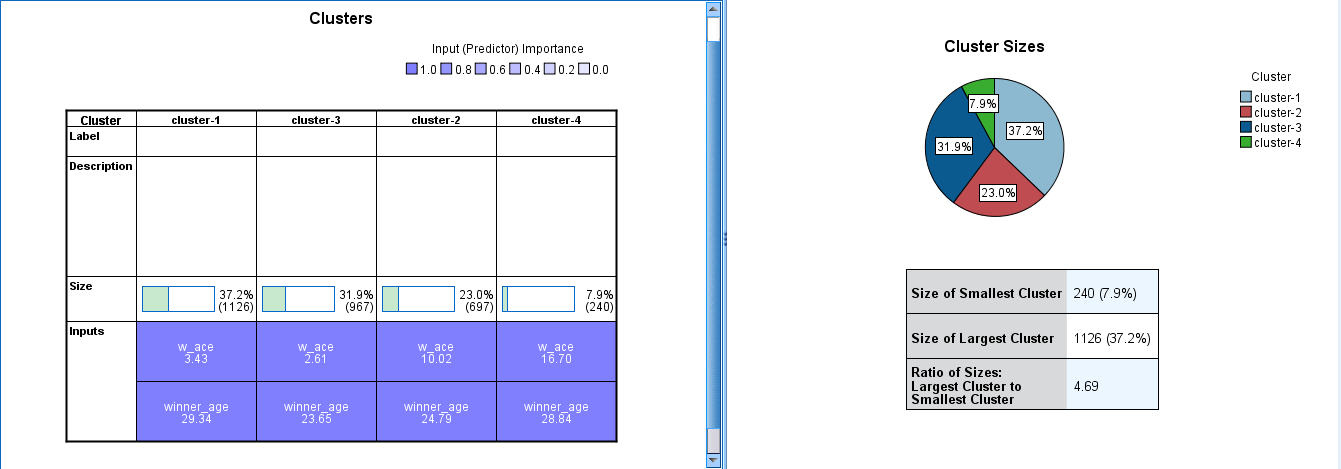
\includegraphics[scale=0.60]{Klasterovanje/Model_KMeans2011.png}
		\end{center}
		\caption{2011. godina}
		\label{fig:SPSS_Model2011}
	\end{subfigure}
	
	\vspace{0.5cm}
	\begin{subfigure}[h]{\textwidth}
		\begin{center}
			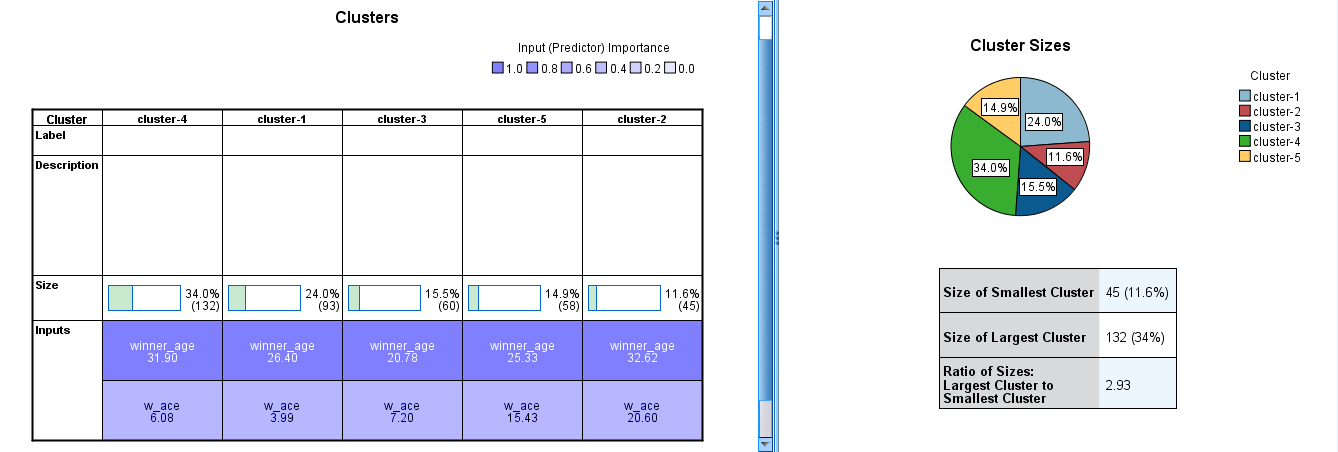
\includegraphics[scale=0.60]{Klasterovanje/Model_KMeans2017.png}
		\end{center}
		\caption{2017. godina}
		\label{fig:SPSS_Model2017}
	\end{subfigure}
	
	\caption{Modeli klastera}
	\label{ModeliKlastera}
\end{figure}

\subsection{KNIME}

\begin{figure}[H]
	\begin{center}
		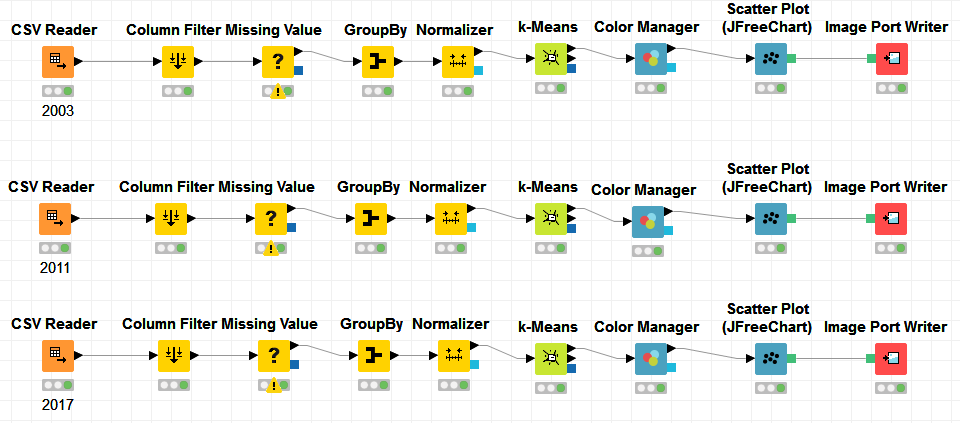
\includegraphics[width=1\textwidth]{Klasterovanje/KNIME_Cvorovi.png}
	\end{center}
	\caption{KNIME klasterovanje}
	\label{fig:KNIME_CvoroviKlasterovanje}
\end{figure}

U fazi pretprocesiranja podataka, otkrili smo jednog igrača sa nepoznatim brojem godina i taj red smo obrisali. U situaciji kada je broj asova bio nepoznat, stavljali smo vrednost nula. Nakon toga smo grupisali podatke po igračima, kako bi za svakog igrača dobili prosek koliko je imao asova tokom godine. Da bi iskoristili \textit{K-Means} algoritam, normalizovali smo podatke kako bi broj godina i broj asova imali isti uticaj na računanje rastojanja među instancama.  

U KNIME-u smo se opredelili da klasterovanje vršimo sa istim brojem klastera kao što smo činili u SPSS-u. Dobijeni klasteri su prikazani na slikama \ref{fig:KNIME_ScatterPlot2003}, \ref{fig:KNIME_ScatterPlot2011} i \ref{fig:KNIME_ScatterPlot2017}.

\begin{figure}[H]
	\begin{center}
		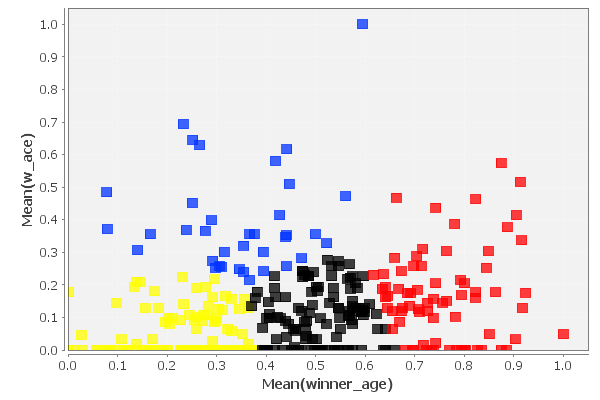
\includegraphics[width=1\textwidth]{Klasterovanje/ScatterPlot_KMeans2003.png}
	\end{center}
	\caption{Klasteri - 2003. godina}
	\label{fig:KNIME_ScatterPlot2003}
\end{figure}
\begin{figure}[H]
	\begin{center}
		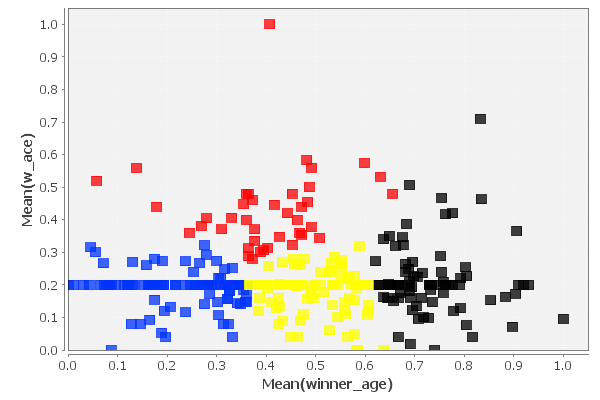
\includegraphics[width=1\textwidth]{Klasterovanje/ScatterPlot_KMeans2011.png}
	\end{center}
	\caption{Klasteri - 2011. godina}
	\label{fig:KNIME_ScatterPlot2011}
\end{figure}
\begin{figure}[H]
	\begin{center}
		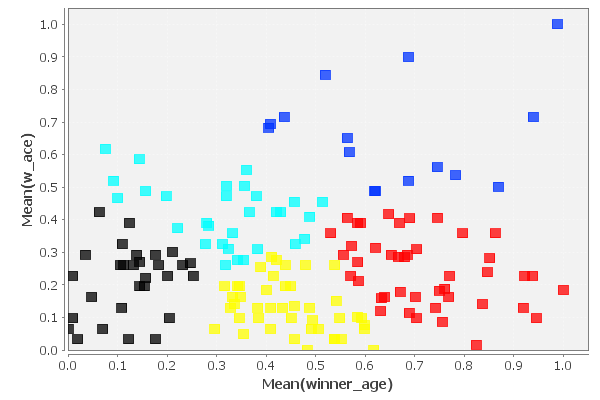
\includegraphics[width=1\textwidth]{Klasterovanje/ScatterPlot_KMeans2017.png}
	\end{center}
	\caption{Klasteri - 2017. godina}
	\label{fig:KNIME_ScatterPlot2017}
\end{figure}

Možemo primetiti da stvarno postoje elementi van granica koji su uticali na to da se formiraju novi klasteri. Igrači koji predstavljaju elemente van granica su dati na slici \ref{fig:IgraciAutlajeri}. 

\begin{figure}[H]
	\begin{subfigure}[h]{\textwidth}
		\begin{center}
			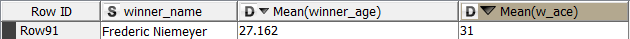
\includegraphics[width=1\textwidth]{Klasterovanje/FredericNiemeyer2003Outlier.png}
		\end{center}
		\caption{2003. godina}
		\label{fig:Autlajer2003}
	\end{subfigure}
	
	\vspace{0.5cm}
	\begin{subfigure}[h]{\textwidth}
		\begin{center}
			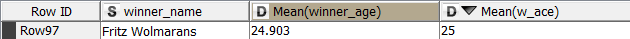
\includegraphics[width=1\textwidth]{Klasterovanje/FritzWolmarans2011Outlier.png}
		\end{center}
		\caption{2011. godina}
		\label{fig:Autlajer2011}
	\end{subfigure}
	
	\vspace{0.5cm}
	\begin{subfigure}[h]{\textwidth}
		\begin{center}
			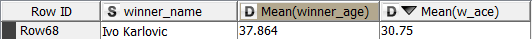
\includegraphics[width=1\textwidth]{Klasterovanje/IvoKarlovic2017Outlier.png}
		\end{center}
		\caption{2017. godina}
		\label{fig:Autlajer2011}
	\end{subfigure}
	
	\caption{Elementi van granica}
	\label{fig:IgraciAutlajeri}
\end{figure} 

Najinteresantiji je definitivno Ivo Karlović, koji je na meču protiv Orasia Zebaljosa na Australian Open-u postigao 75 asova. Treba imati na umu da je Karlović odigrao četiri meča na ovom turniru. Moramo napomenuti, da je skup podataka o 2017. godini nepotpun, jer je u toku te godine napravljen skup i da dosta turnira još uvek nije upisano. Trenutni skup ima samo podatke sa turnira odigranih u januaru i februaru.  


\section{Klasifikacija}

Za klasifikaciju smo odlučili da nam klase budu podloge terena, a pripadnost svakoj klasi se određuje na osnovu karakteristika četiri gubitnikova atributa (broj asova gubitnika, broj duplih servis grešaka gubitnika, broj ubačenih prvih servisa gubitnika, broj brejk šansi na servis gubitnika). Kao i kod klasterovanja i ovde smo želeli da vidimo šta se dešava u više godina. S obzirom na to da su neke podloge prisutnije u odnosu na ostale. Nakon detaljne analize raspodele podloga, odlučili smo se za 2005., 2008. i 2015. godinu. Razlog što smo odabrali baš ove godine jeste polako gubljenje ˝tepiha˝ kao podloge (slike \ref{fig:Podloga2005}, \ref{fig:Podloga2008} i \ref{fig:Podloga2015}), pa nas je zanimalo kako će ova činjenica uticati na sam proces klasifikacije. 

\begin{figure}[H]
	\begin{center}
		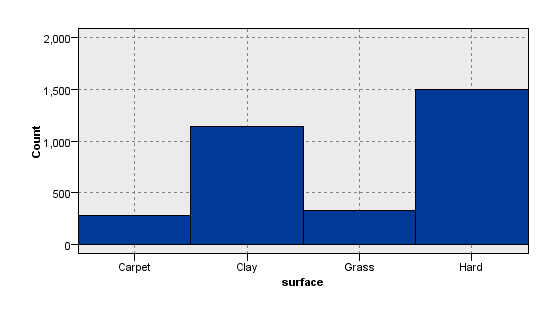
\includegraphics[width=0.7\textwidth]{Klasifikacija/HistogramiPodlogaTerena/Graphboard2005.png}
	\end{center}
	\caption{Podloga - 2005. godina}
	\label{fig:Podloga2005}
\end{figure}

\newgeometry{top=5.5cm}
\begin{figure}[H]
	\begin{center}
		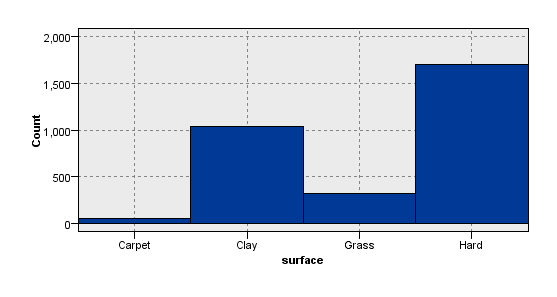
\includegraphics[width=0.7\textwidth]{Klasifikacija/HistogramiPodlogaTerena/Graphboard2008.png}
	\end{center}
	\caption{Podloga - 2008. godina}
	\label{fig:Podloga2008}
\end{figure}
\begin{figure}[H]
	\begin{center}
		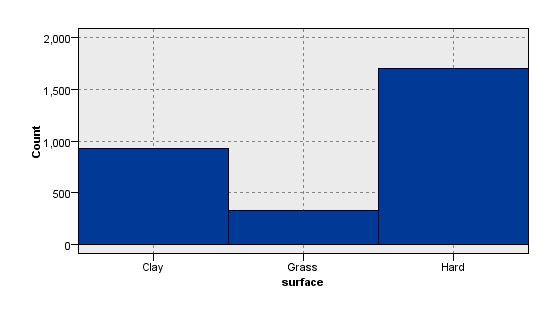
\includegraphics[width=0.7\textwidth]{Klasifikacija/HistogramiPodlogaTerena/Graphboard2015.png}
	\end{center}
	\caption{Podloga - 2015. godina}
	\label{fig:Podloga2015}
\end{figure}

Klasifikaciju smo, takođe, obradili u SPSS-u i u KNIME-u.

\restoregeometry
\subsection{SPSS}

\begin{figure}[H]
	\begin{center}
		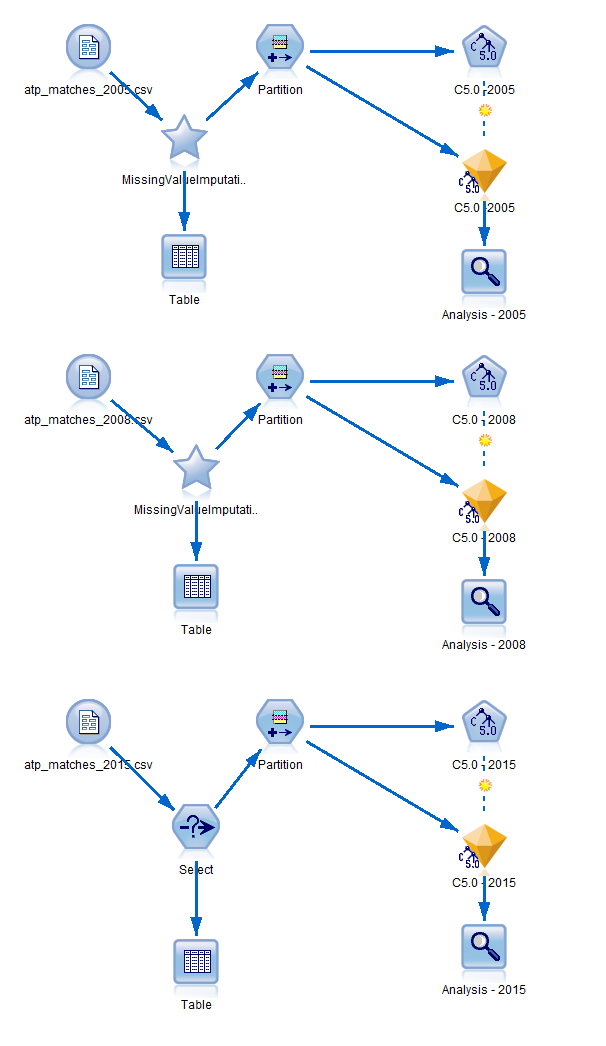
\includegraphics[width=0.7\textwidth]{Klasifikacija/C50/SPSS_C50_Surface.png}
	\end{center}
	\caption{SPSS klastifikacija}
	\label{fig:SPSS_CvoroviKlasifikacija}
\end{figure}

Primenili smo \textit{C5.0} algoritam sa podelom na trening i test skup u odnosu 70-30. Na slici \ref{fig:ModelKlasifikacijaC50} možemo videti analizu najvažnijjih atributa. Najvažniji atribut u 2008. i 2015. godini je broj asova, dok u 2005. godini broj asova zauzima treće mesto po važnosti. Ono što je interesantno jeste da se u 2005. godini broj duplih servis grešaka smatra najvažnijim, dok se u 2008. i 2015. godini može videti da je važnost ovog atributa skoro nula, 0.03 i 0.09 respektivno.

\newgeometry{top=5.0cm}
\begin{figure}[H]
	\begin{subfigure}[h]{\textwidth}
		\begin{center}
			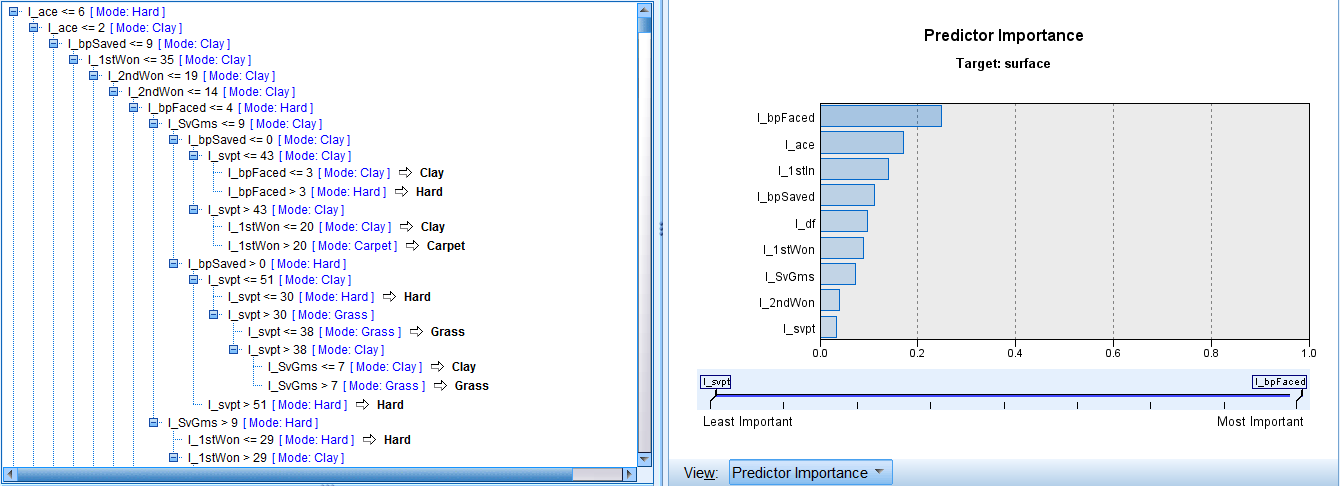
\includegraphics[width=0.9\textwidth]{Klasifikacija/C50/Model_Surface2005.png}
		\end{center}
		\caption{2005. godina}
		\label{fig:ModelKlasifikacijaC502005}
	\end{subfigure}
	
	\vspace{0.5cm}
	\begin{subfigure}[h]{\textwidth}
		\begin{center}
			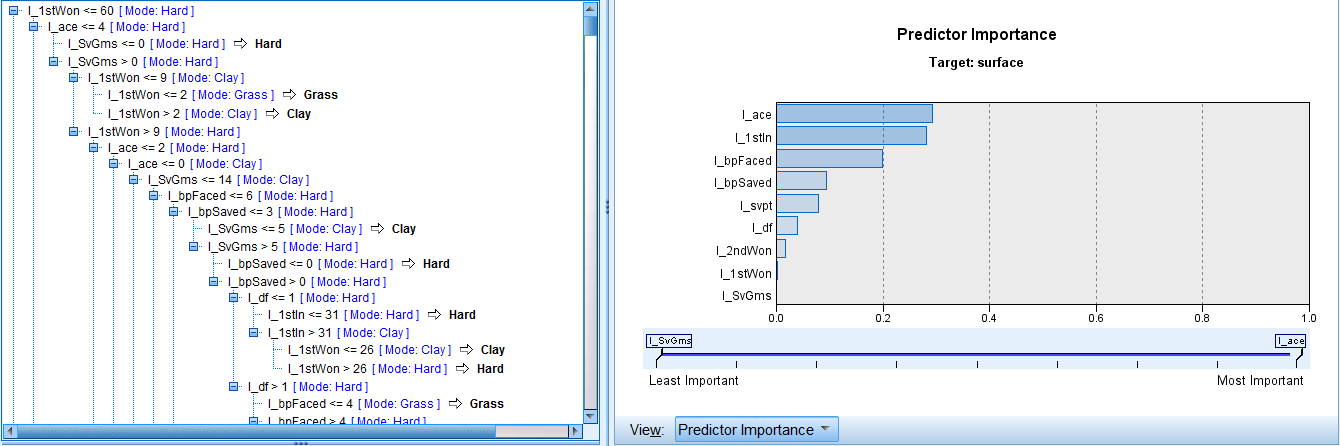
\includegraphics[width=0.9\textwidth]{Klasifikacija/C50/Model_Surface2008.png}
		\end{center}
		\caption{2008. godina}
		\label{fig:ModelKlasifikacijaC502008}
	\end{subfigure}
	
	\vspace{0.5cm}
	\begin{subfigure}[h]{\textwidth}
		\begin{center}
			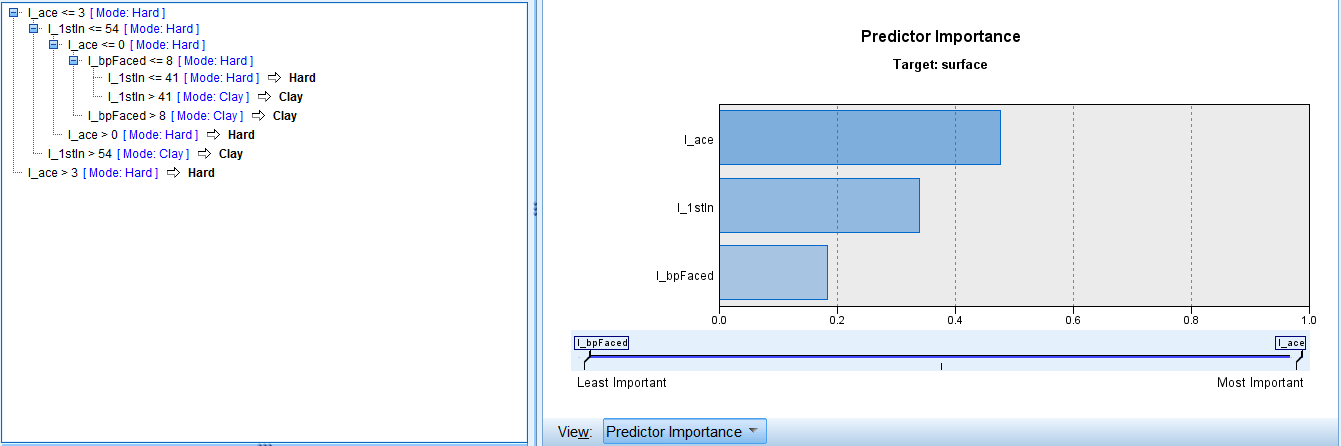
\includegraphics[width=0.9\textwidth]{Klasifikacija/C50/Model_Surface2015.png}
		\end{center}
		\caption{2015. godina}
		\label{fig:ModelKlasifikacijaC502015}
	\end{subfigure}
	
	\caption{Model klasifikacije}
	\label{fig:ModelKlasifikacijaC50}
\end{figure}

Neke segmente drveta odlučivanja smo mogli da vidimo i na prethodnoj slici, a detaljniji prikaz se može pogledati na sledećim linkovima: \href{file:./Klasifikacija/C50/Model_Surface2005.html}{2005}, \href{file:./Klasifikacija/C50/Model_Surface2008.html}{2008}, \href{file:./Klasifikacija/C50/Model_Surface2015.html}{2015}. 

\restoregeometry
Intuitivan prikaz drveta odlučivanja za sve godine se može videti na slici \ref{fig:DrvoOdlucivanjaC50}.

\begin{figure}[H]
	\begin{subfigure}[h]{\textwidth}
		\begin{center}
			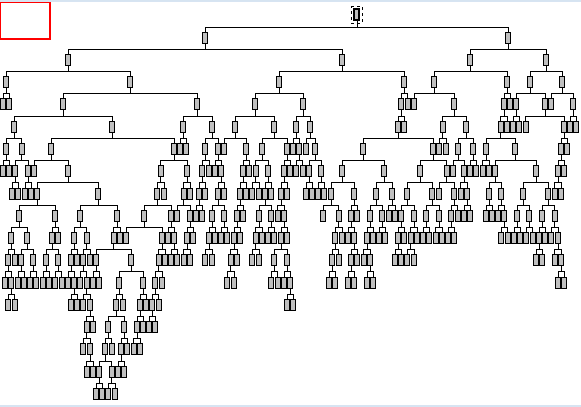
\includegraphics[scale=0.70]{Klasifikacija/C50/MapaDrvetaOdlucivanja2005.png}
		\end{center}
		\caption{2005. godina}
		\label{fig:DrvoOdlucivanjaC502005}
	\end{subfigure}

	\vspace{0.5cm}
	\begin{subfigure}[h]{\textwidth}
		\begin{center}
			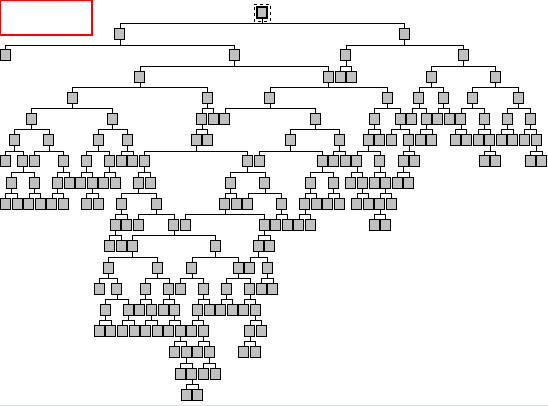
\includegraphics[scale=0.70]{Klasifikacija/C50/MapaDrvetaOdlucivanja2008.png}
		\end{center}
		\caption{2008. godina}
		\label{fig:DrvoOdlucivanjaC502008}
	\end{subfigure}
	
	\vspace{0.5cm}
	\begin{subfigure}[h]{\textwidth}
		\begin{center}
			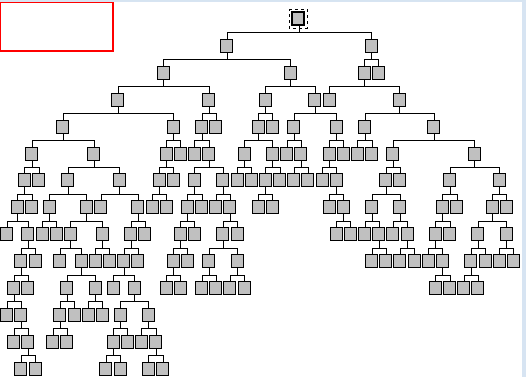
\includegraphics[scale=0.70]{Klasifikacija/C50/MapaDrvetaOdlucivanja2015.png}
		\end{center}
		\caption{2015. godina}
		\label{fig:DrvoOdlucivanjaC502015}
	\end{subfigure}
	
	\caption{Drveta odlučivanja dobijena algoritmom C-5.0}
	\label{fig:DrvoOdlucivanjaC50}
\end{figure}

Kao što možemo da vidimo, drveta su veoma duboka i razgranata. Na slici \ref{fig:MatricaKnfuzijeC50} se može videti da je dobijena preciznost na trening skupu manja od 70\%, dok je na test skupu ta preciznost oko 50\%. 

\begin{figure}[H]
	\begin{subfigure}[h]{\textwidth}
		\begin{center}
			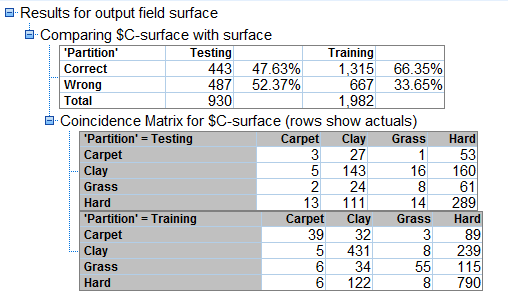
\includegraphics[width=0.7\textwidth]{Klasifikacija/C50/Analysis_Surface2005.png}
		\end{center}
		\caption{2005. godina}
		\label{fig:MatricaKnfuzijeC502005}
	\end{subfigure}
	\vspace{0.2cm}
	\begin{subfigure}[h]{\textwidth}
		\begin{center}
			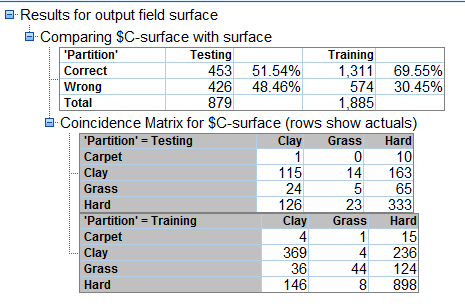
\includegraphics[width=0.7\textwidth]{Klasifikacija/C50/Analysis_Surface2008.png}
		\end{center}
		\caption{2008. godina}
		\label{fig:MatricaKnfuzijeC502008}
	\end{subfigure}
	\vspace{0.2cm}
	\begin{subfigure}[h]{\textwidth}
		\begin{center}
			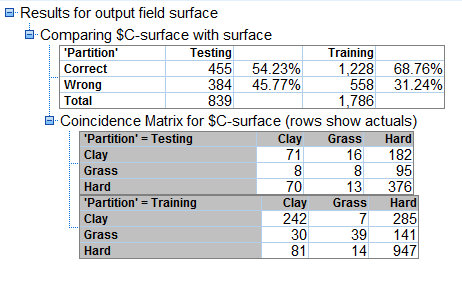
\includegraphics[width=0.7\textwidth]{Klasifikacija/C50/Analysis_Surface2015.png}
		\end{center}
		\caption{2015. godina}
		\label{fig:MatricaKnfuzijeC502015}
	\end{subfigure}
	\caption{Matrice konfuzije - C5.0}
	\label{fig:MatricaKnfuzijeC50}
\end{figure}

\newgeometry{top=3.5cm}
Možemo da primetimo da se ˝tepih˝ klasifikuje kao ˝beton˝, što je i očekivano s obzirom da se najviše turnira igra na betonu. 

Sveobuhvatni prikaz rada algoritma \textit{C5.0} dat je u fajlovima: \href{file:./Klasifikacija/C50/Summary_Surface2005.html}{2005}, \href{file:./Klasifikacija/C50/Summary_Surface2008.html}{2008}, \href{file:./Klasifikacija/C50/Summary_Surface2005.html}{2015}.  

S obzirom da nismo bili zadovoljni rezultatima dobijenim algoritmom \textit{C5.0}, kao i to da nam je dobijena preciznost na trening i test skupu ukazivala da je možda došlo do preprilagođavanja, odlučili smo da na 2005. i 2015. godinu izvršimo istu analizu u alatu KNIME. Još jedan od razloga za istraživanje podataka u drugom alatu, bio je i taj što smo želili moguće izvršiti odsecanje drveta ranije u toku grananja.

\subsection{KNIME}

U alatu KNIME smo za klasifikaciju koristili Drveta odlučivanja, K najbližih suseda i metod potpornih vektora (SVM). Podatke smo takođe podelili na trening i test skup u odnosu 70-30.

\subsubsection{Drveta odlučivanja}

\begin{figure}[H]
	\begin{center}
		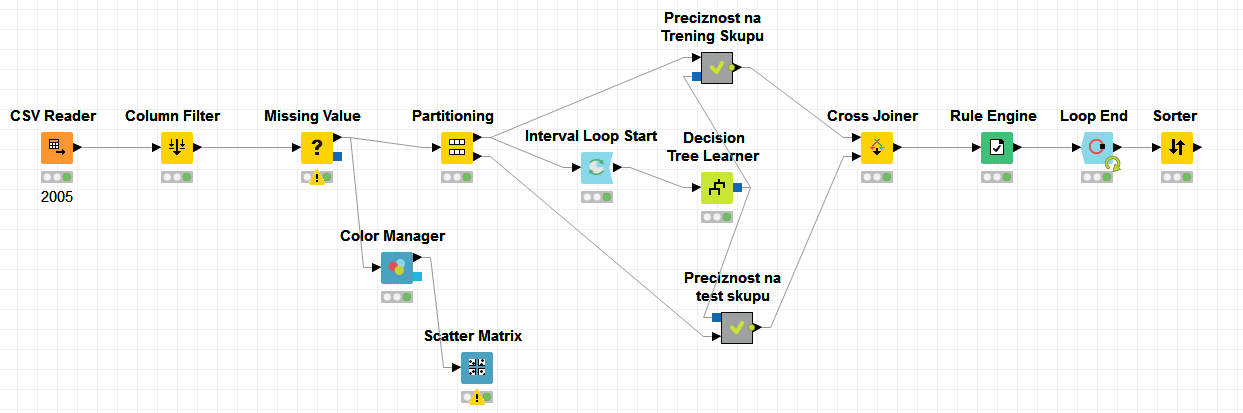
\includegraphics[width=\textwidth]{Klasifikacija/DrvoOdlucivanja/KNIME_DrvoOdlucivanjaCvorovi.png}
	\end{center}
	\caption{KNIME implementacija tehnike Drveta odlučivanja}
	\label{fig:KNIME_CvoroviKlasifikacija}
\end{figure}

Pre same klasifikacije, na slikama \ref{fig:KlasifikacijaScatterMatrix2005} i \ref{fig:KlasifikacijaScatterMatrix2015} je prikazan odnos između nekih atributa po kojima je vršena klasifikacija. Možemo primetiti tesnu povezanost između broja asova i broj ubačenih prvih servisa gubitnika. 

\begin{figure}[H]
	\begin{center}
		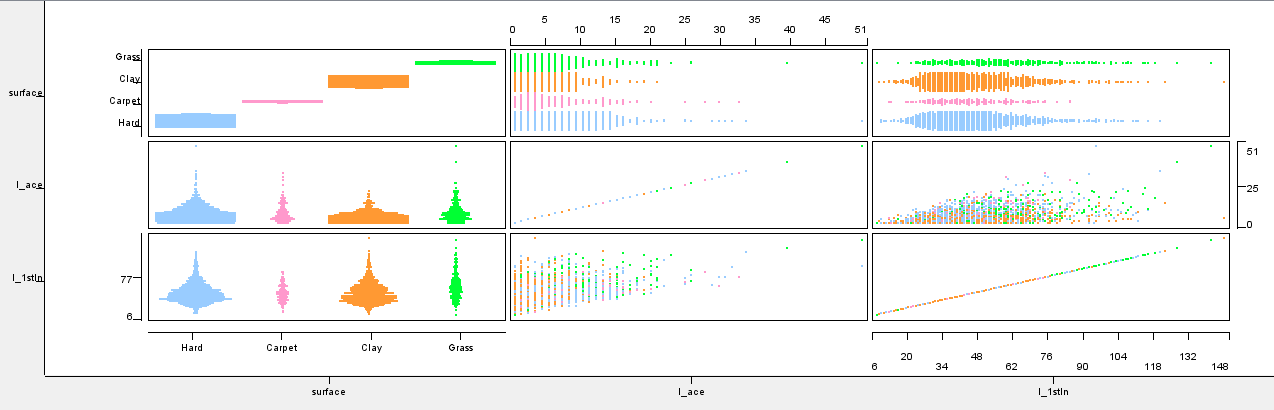
\includegraphics[width=\textwidth]{Klasifikacija/DrvoOdlucivanja/2005/KorelacijaAsInSurface.png}
	\end{center}
	\caption{ Korelacija atributa - 2005. godina}
	\label{fig:KlasifikacijaScatterMatrix2005}
\end{figure}
\restoregeometry
\begin{figure}[H]
	\begin{center}
		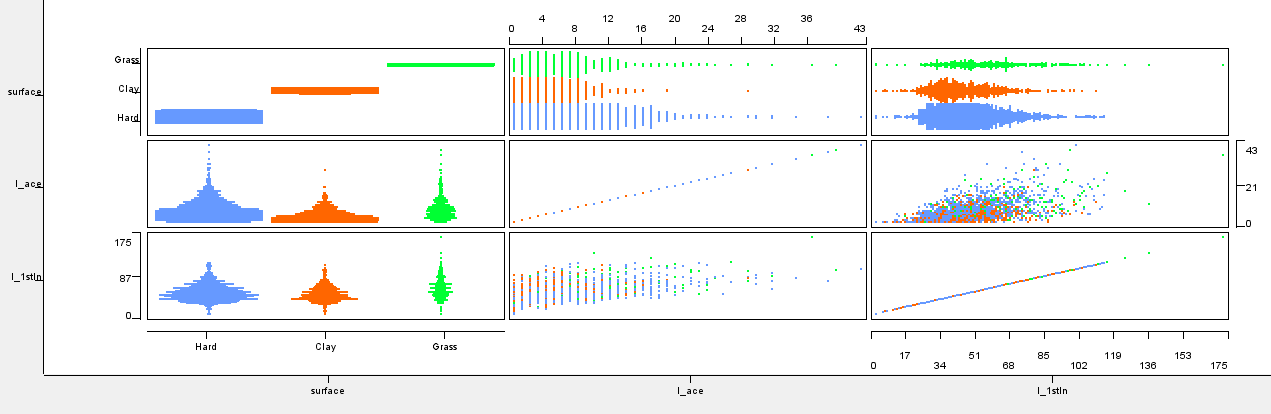
\includegraphics[width=\textwidth]{Klasifikacija/DrvoOdlucivanja/2015/KorelacijaAsInSurface.png}
	\end{center}
	\caption{ Korelacija atributa - 2015. godina}
	\label{fig:KlasifikacijaScatterMatrix2015}
\end{figure}

Dobijene matrice konfuzije su prikazane na slikama \ref{fig:MatricaKnfuzije2005} i \ref{fig:MatricaKnfuzije2015}.
Za 2005. godinu, i na trening i na test skupu vidimo da se tepih i trava klasifikuju pre svega kao beton, a potom i kao šljaka.
Za 2015. godinu, i na trening i na test skupu vidimo da se trava i dalje klasifikuje uglavnom kao beton.

\begin{figure}[H]
	\begin{subfigure}[h]{\textwidth}
		\begin{center}
			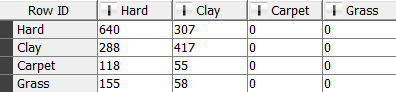
\includegraphics[width=0.6\textwidth]{Klasifikacija/DrvoOdlucivanja/2005/MatricaKonfuzijeTrening.png}
		\end{center}
		\caption{Trening skup}
		\label{fig:MatricaKnfuzijeTrening2005}
	\end{subfigure}

	\vspace{0.5cm}
	\begin{subfigure}[h]{\textwidth}
		\begin{center}
			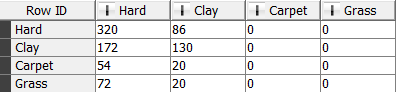
\includegraphics[width=0.6\textwidth]{Klasifikacija/DrvoOdlucivanja/2005/MatricaKonfuzijeTest.png}
		\end{center}
		\caption{Test skup}
		\label{fig:MatricaKnfuzijeTest2005}
	\end{subfigure}
	\caption{Matrice konfuzije - 2005}
	\label{fig:MatricaKnfuzije2005}
\end{figure}

\begin{figure}[H]
	\begin{subfigure}[h]{\textwidth}
		\begin{center}
			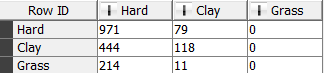
\includegraphics[width=0.6\textwidth]{Klasifikacija/DrvoOdlucivanja/2015/MatricaKonfuzijeTrening.png}
		\end{center}
		\caption{Trening skup}
		\label{fig:MatricaKnfuzijeTrening2015}
	\end{subfigure}

	\vspace{0.5cm}
	\begin{subfigure}[h]{\textwidth}
		\begin{center}
			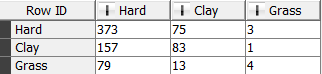
\includegraphics[width=0.6\textwidth]{Klasifikacija/DrvoOdlucivanja/2015/MatricaKonfuzijeTest.png}
		\end{center}
		\caption{Test skup}
		\label{fig:MatricaKnfuzijeTest2015}
	\end{subfigure}
	\caption{Matrice konfuzije - 2015}
	\label{fig:MatricaKnfuzije2015}
\end{figure}

Preciznost se može videti na slici \ref{fig:PreciznostKNIME}.
Da bismo dobili što bolju preciznost, primenili smo algoritam za vrednosti od 5 do 100 sa korakom 5 za minimalni broj podloga po čvoru u drvetu odlučivanja.
Primetimo da je najveća preciznost na trening i test skupu u 2005. godini dobijena u rasponu od 5 do 15 podloga po čvoru.
Isti princip smo primenili i za 2015. godinu i dobili da je preciznost na test skupu najveća za vrednosti u rasponu od 45 do 60 podloga po čvoru.

Korišćenjem ovog alata, nismo dobili značajnu razliku u odnosu na preciznost dobijenu u alatu SPSS, ali je primetna razlika u dubini drveta odlučivanja, što se može videti na slikam \ref{fig:DrvoOdlucivanja2005} i \ref{fig:DrvoOdlucivanja2015}. Kao meru nečistoće koristili smo Ginijev indeks i MDL metod za odsecanje stabla.

\begin{figure}[H]
	\begin{subfigure}[h]{\textwidth}
		\begin{center}
			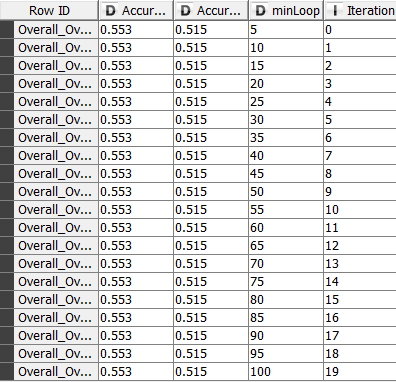
\includegraphics[width=0.6\textwidth]{Klasifikacija/DrvoOdlucivanja/2005/Preciznost.png}
		\end{center}
		\caption{2005. godina}
		\label{fig:Preciznost2005}
	\end{subfigure}
	
	\vspace{0.5cm}
	\begin{subfigure}[h]{\textwidth}
		\begin{center}
			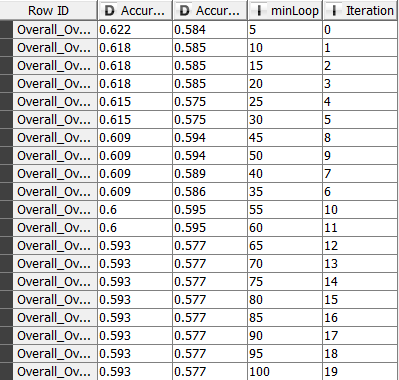
\includegraphics[width=0.6\textwidth]{Klasifikacija/DrvoOdlucivanja/2015/Preciznost.png}
		\end{center}
		\caption{2015. godina}
		\label{fig:Preciznost2015}
	\end{subfigure}
	
	\caption{Preciznost}
	\label{fig:PreciznostKNIME}
\end{figure}

\begin{figure}[H]
	\begin{center}
		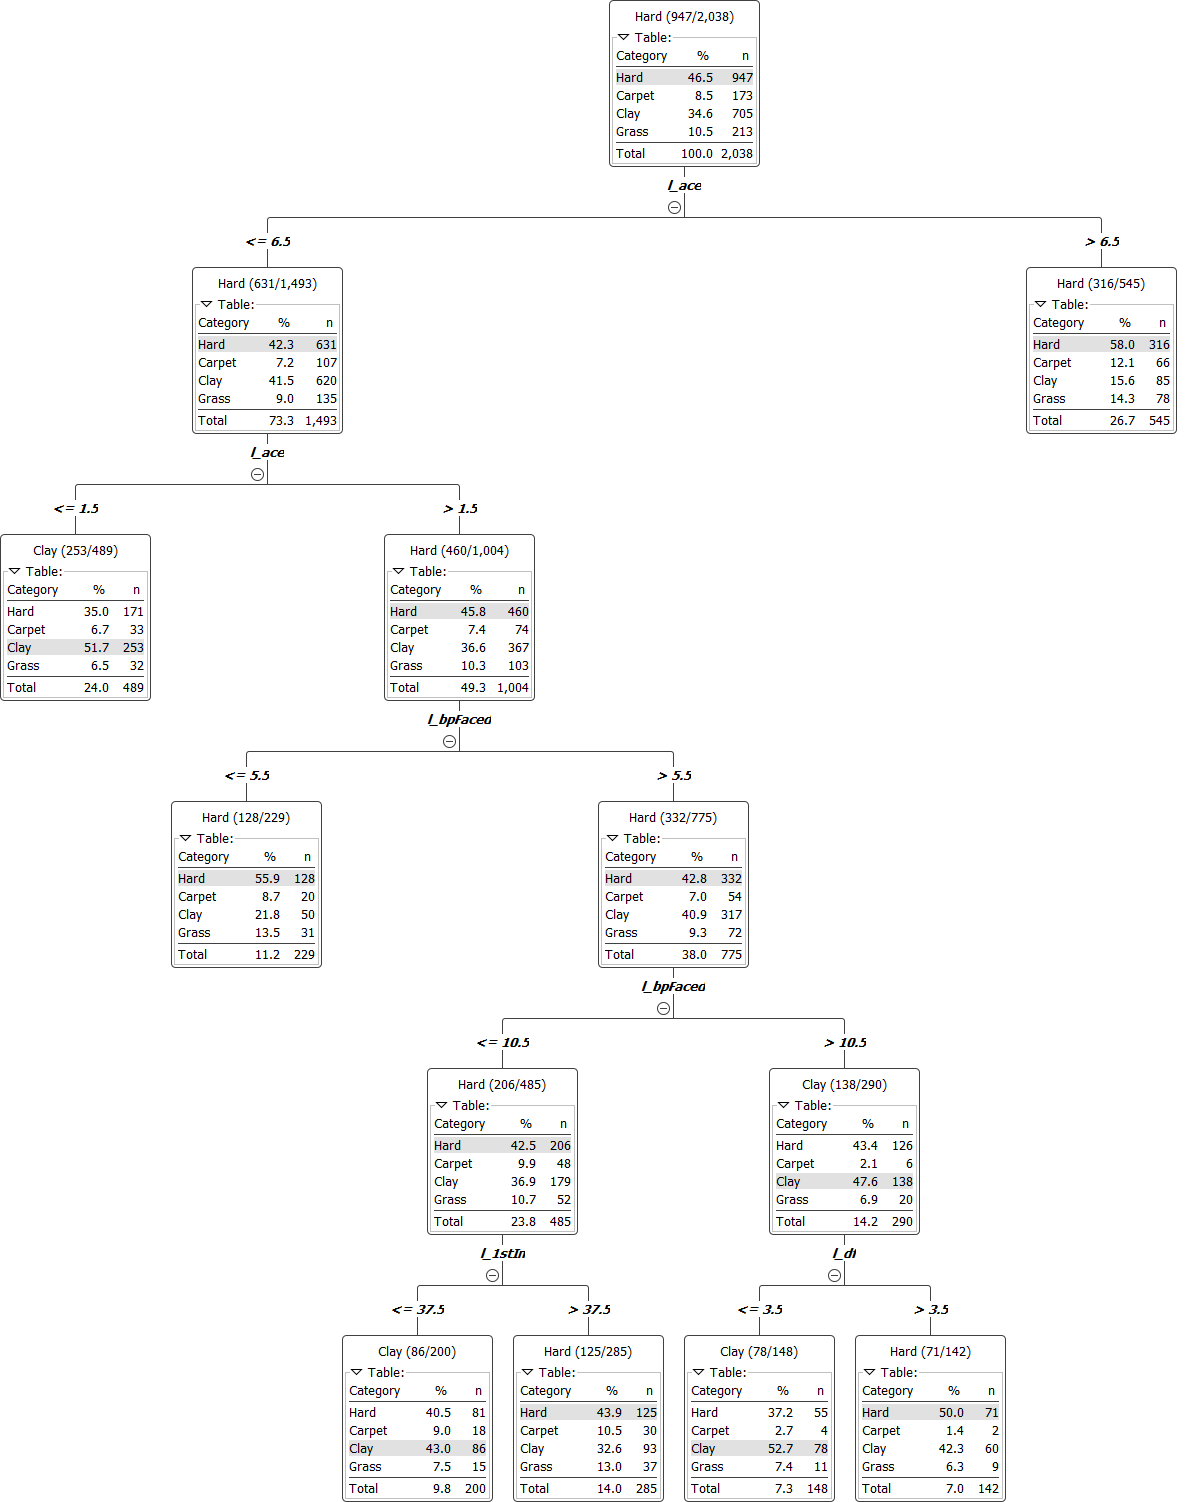
\includegraphics[width=\textwidth]{Klasifikacija/DrvoOdlucivanja/2005/DrvoOdlucivanja.png}
	\end{center}
	\caption{Ginijev indeks - 2005. godina}
	\label{fig:DrvoOdlucivanja2005}
\end{figure}
\begin{figure}[H]
	\begin{center}
		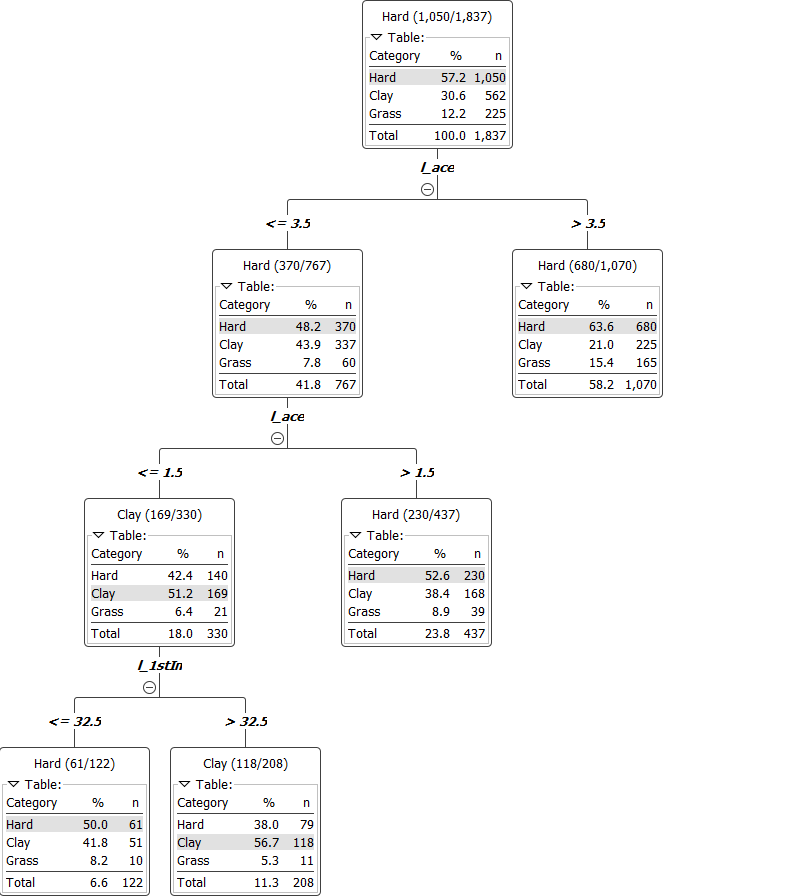
\includegraphics[width=\textwidth]{Klasifikacija/DrvoOdlucivanja/2015/DrvoOdlucivanja.png}
	\end{center}
	\caption{Ginijev indeks - 2015. godina}
	\label{fig:DrvoOdlucivanja2015}
\end{figure}

\subsubsection{K najbližih suseda}

\begin{figure}[H]
	\begin{center}
		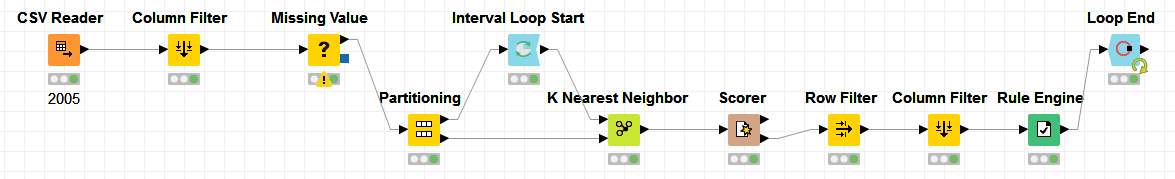
\includegraphics[width=\textwidth]{Klasifikacija/kNN/KNIME_kNNCvorovi.png}
	\end{center}
	\caption{KNIME implementacija tehnike k najbližih suseda}
	\label{fig:KNIME_CvorovikNN}
\end{figure}

Koristeći metodu k najbližih suseda, dobili smo slične rezultate.
Matrice konfuzije su date na slici \ref{fig:MatricaKonfuzije}.

\begin{figure}[H]
	\begin{subfigure}[h]{\textwidth}
		\begin{center}
			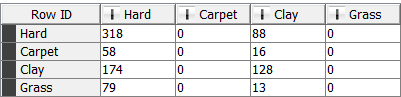
\includegraphics[width=0.6\textwidth]{Klasifikacija/kNN/MatricaKonfuzije2005.png}
		\end{center}
		\caption{2005. godina}
		\label{fig:MatricaKnfuzijeg2005}
	\end{subfigure}
	
	\vspace{0.5cm}
	\begin{subfigure}[h]{\textwidth}
		\begin{center}
			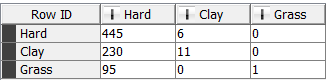
\includegraphics[width=0.6\textwidth]{Klasifikacija/kNN/MatricaKonfuzije2015.png}
		\end{center}
		\caption{2015. godina}
		\label{fig:MatricaKnfuzijeg2015}
	\end{subfigure}
	\caption{Matrice konfuzije}
	\label{fig:MatricaKonfuzije}
\end{figure}

Preciznost smo izračunali za vrednosti k u rasponu od 3 do 100 sa korakom 1. Na slikama \ref{fig:PreciznostKNN2005} i \ref{fig:PreciznostKNN2015} se može videti
da je najbolja preciznost na test skupu dobijena za 2005. godinu, za k=35 i iznosi 0.527.
U 2015. godini, najveća preciznost na test skupu je dobijena za vrednost k=47 i iznosi 0.589.

\begin{figure}[H]
	\begin{center}
		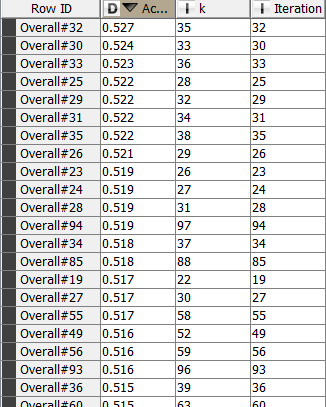
\includegraphics[width=0.6\textwidth]{Klasifikacija/kNN/Preciznost2005.png}
	\end{center}
	\caption{Preciznost kNN - 2005. godina}
	\label{fig:PreciznostKNN2005}
\end{figure}
\begin{figure}[H]
	\begin{center}
		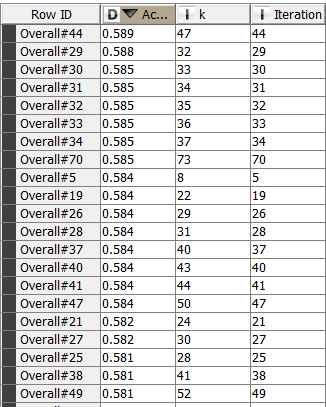
\includegraphics[width=0.6\textwidth]{Klasifikacija/kNN/Preciznost2015.png}
	\end{center}
	\caption{Preciznost kNN - 2015. godina}
	\label{fig:PreciznostKNN2015}
\end{figure}

Dobijeni rezultati su približno isti kao i preciznosti dobijene na test skupu metodom drveta odlučivanja. Prikazaćemo rezultate koje smo dobili još metodom SVM.

\subsubsection{SVM}

\begin{figure}[H]
	\begin{center}
		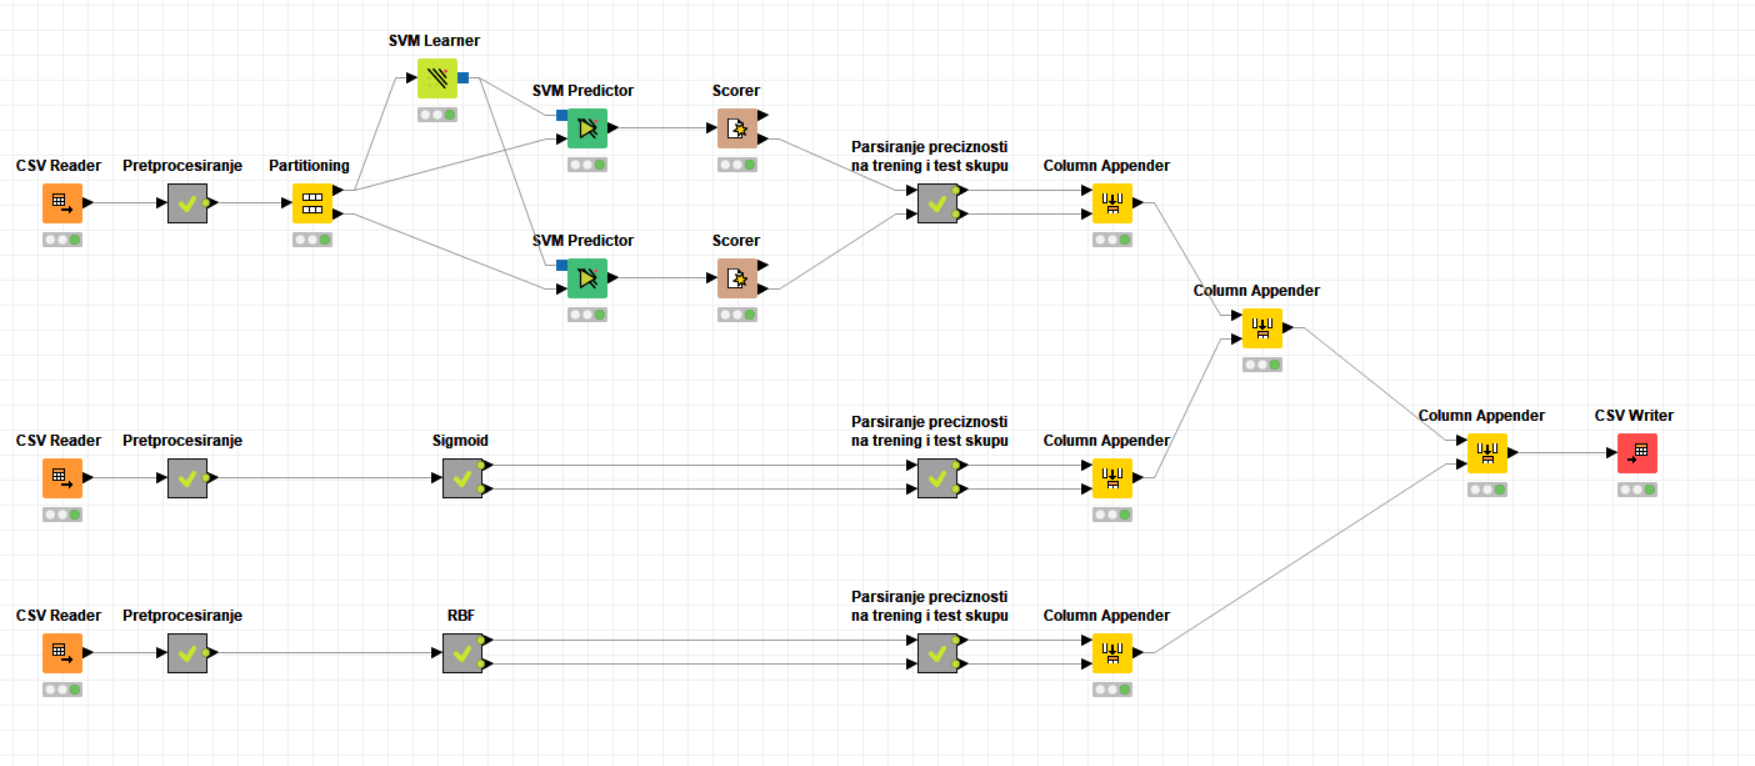
\includegraphics[width=1\textwidth]{Klasifikacija/SVM/SVM_knime}
	\end{center}
	\caption{KNIME implementacija SVM tehnike}
	\label{fig:KNIME_CvoroviKlasifikacija}
\end{figure}

Na normalizovanim podacima, primenili smo sva tri raspoloživa kernela (polinomijalni trećeg stepena, sigmoid, Gausov(RBF)) za 2005. godinu.
Na slici \ref{fig:precision} se mogu videti preciznosti za sva tri kernela, i za trening i za test skup.

\begin{figure}[H]
	\begin{center}
		
\includegraphics[width=1\textwidth]{Klasifikacija/SVM/preciznostSlika.png}
	\end{center}
	\caption{Preciznost za različite kernele}
	\label{fig:precision}
\end{figure}


Koristeći polinomijalni kernel trećeg stepena, dobili smo izuzetno loše rezultate.
Naime, skoro 50\% redova (1501 od 3257) odgovaraju mečevima koji su odigrani na tvrdoj podlozi.
Na slikama \ref{fig:poly_training} i \ref{fig:poly_test} vidimo da su podaci pogrešno klasifikovani u
mečeve koji su odigrani na šljaci.

\begin{figure}[H]
	\begin{center}
		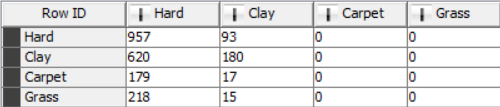
\includegraphics[width=0.6\textwidth]{Klasifikacija/SVM/poly_training}
	\end{center}
	\caption{Trening podaci za polinomijalni kernel}
	\label{fig:poly_training}
\end{figure}

\begin{figure}[H]
	\begin{center}
		\includegraphics[width=0.6\textwidth]{Klasifikacija/SVM/poly_test}
	\end{center}
	\caption{Test podaci za polinomijalni kernel}
	\label{fig:poly_test}
\end{figure}

%\newpage

Koristeći sigmoid kernel, situacija se promenila utoliko što su podaci vezani za tvrdu podlogu
vrlo dobro klasifikovani, što se može videti na slikama \ref{fig:sigmoid_training} i \ref{fig:sigmoid_test}.
Primetimo da su podaci uglavnom raspoređeni u klase koje se odnose na beton, šljaku i tepih.

\begin{figure}[H]
	\begin{center}
		\includegraphics[width=0.6\textwidth]{Klasifikacija/SVM/sigmoid_training}
	\end{center}
	\caption{Trening podaci za sigmoid kernel}
	\label{fig:sigmoid_training}
\end{figure}

\begin{figure}[H]
	\begin{center}
		\includegraphics[width=0.6\textwidth]{Klasifikacija/SVM/sigmoid_test}
	\end{center}
	\caption{Test podaci za sigmoid kernel}
	\label{fig:sigmoid_test}
\end{figure}

Koristeći Gausov kernel, dobili smo lošiju klasifikaciju za tvrdu podlogu, dosta bolju klasifikaciju za šljaku, bolju klasifikaciju za travu, dok
je tepih u potpunosti promašen (slike \ref{fig:rbf_training} i \ref{fig:rbf_test}).\\

\newgeometry{top=10.0cm}
\begin{figure}[H]
	\begin{center}
		\includegraphics[width=0.7\textwidth]{Klasifikacija/SVM/rbf_training}
	\end{center}
	\caption{Trening podaci za Gausov kernel}
	\label{fig:rbf_training}
\end{figure}

\begin{figure}[H]
\begin{center}
	\includegraphics[width=0.7\textwidth]{Klasifikacija/SVM/rbf_test}
\end{center}
\caption{Test podaci za Gausov kernel}
\label{fig:rbf_test}
\end{figure}

\restoregeometry

\end{document}